% Auto-included figure block (draft images regenerated by paper-figure pipeline; paths are git-versioned).
% The PNGs exist in /work1/zixuan/outputs/agent_memory/pilot/{analysis,h3}; camera-ready ships vector PDFs.

\begin{figure}[t]
  \centering
  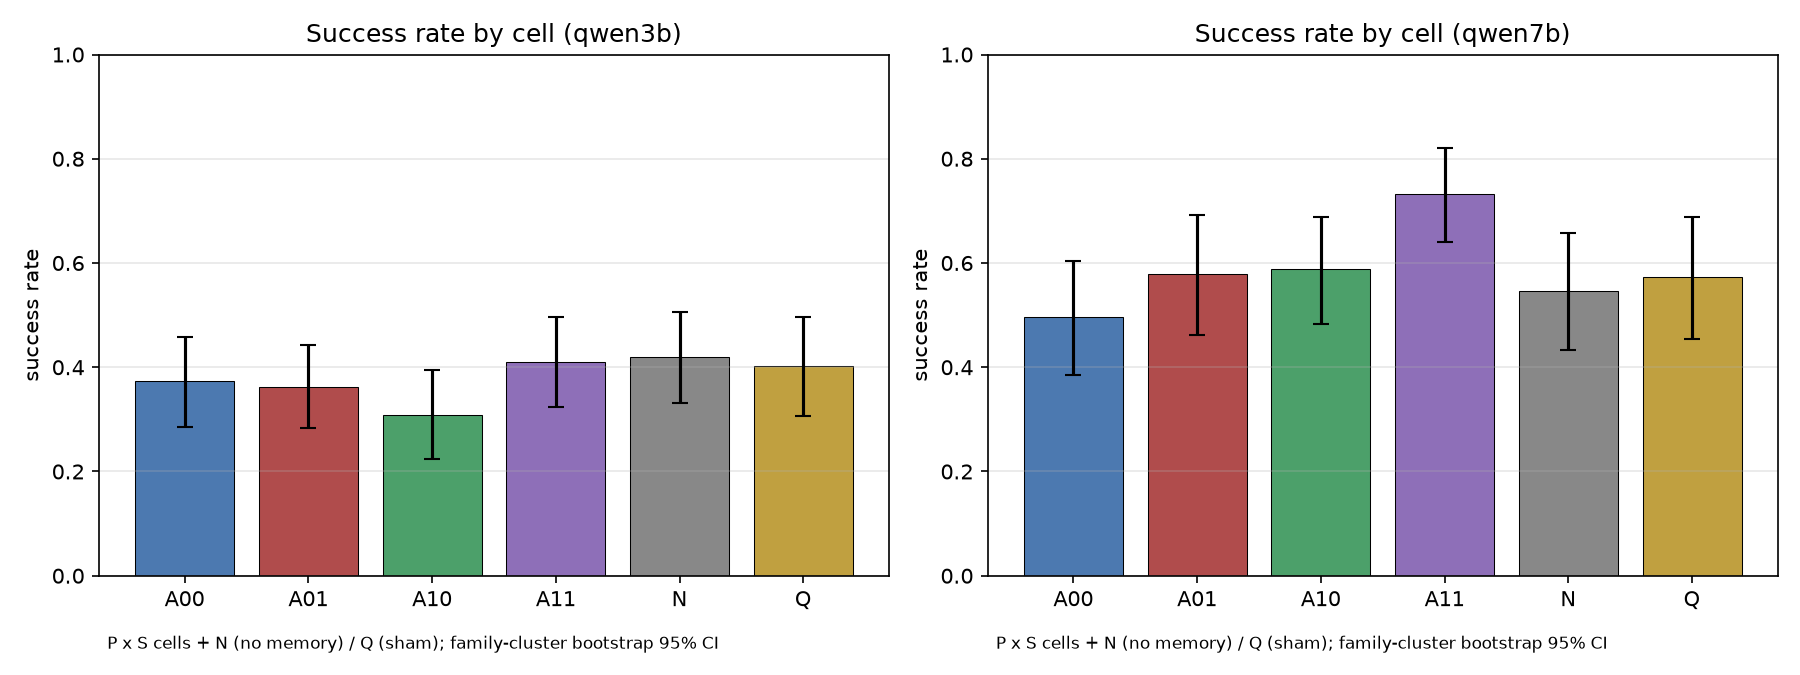
\includegraphics[width=\linewidth]{figs/fig1_cells_success.png}
  \caption{Stage-A cell success rates with 95\% family-cluster CIs. A11 (replay-like) dominates the 7B pooled gain; the 3B pattern differs---only A11 gets near-parity with N while A10 (clean structural) falls below the unrelated control, foreshadowing the scale reversal of Section~\ref{ssec:scale}.}
  \label{fig:fig1}
\end{figure}

\begin{figure}[t]
  \centering
  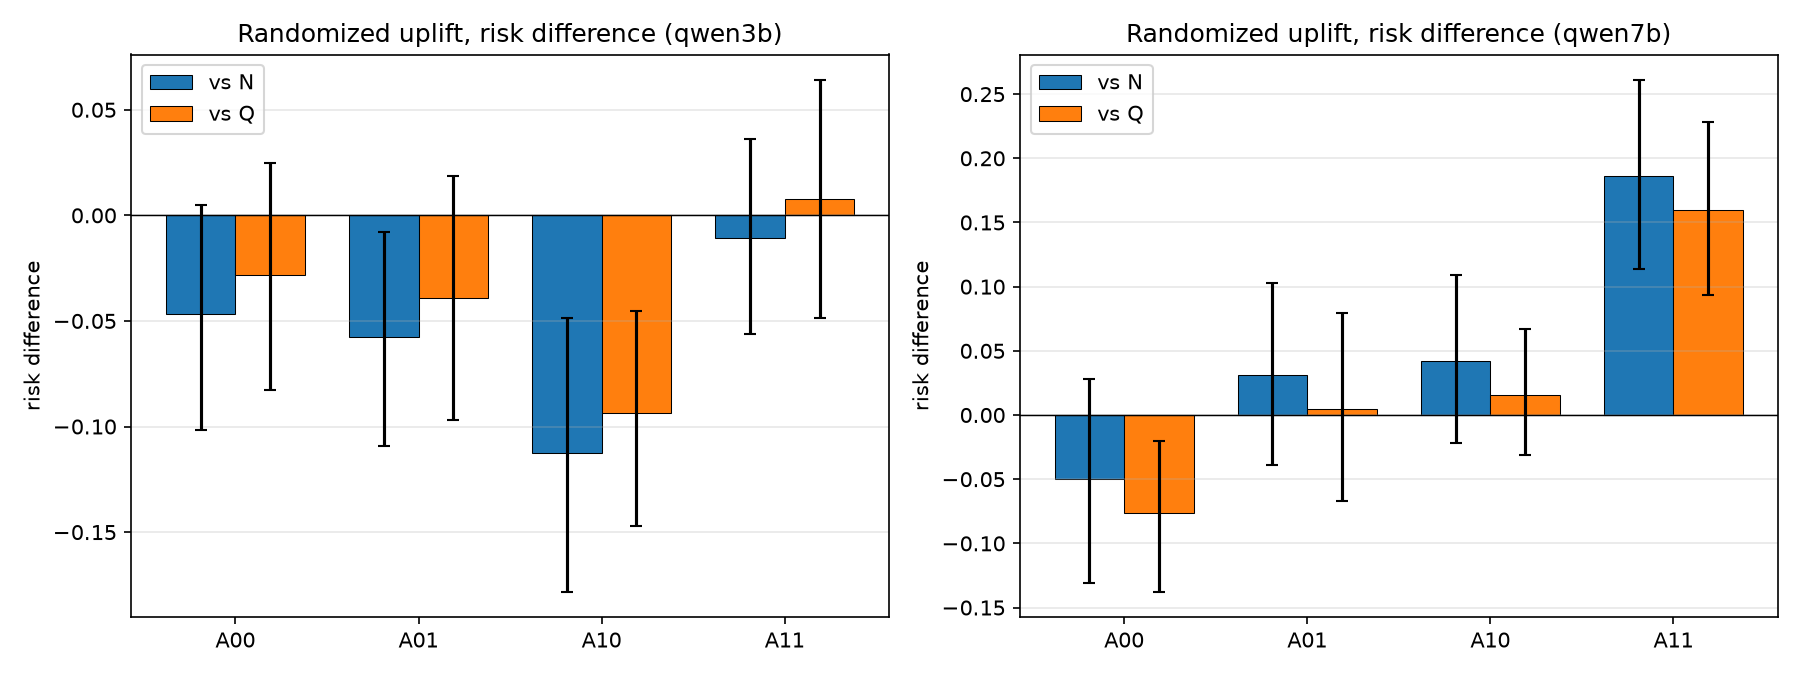
\includegraphics[width=\linewidth]{figs/fig2_uplift.png}
  \caption{Risk differences relative to N and Q. The format/context effect ($Q-N$) hugs zero; the decomposition separates a small structural term from a large replay term; 3B only benefits through A11.}
  \label{fig:fig2}
\end{figure}

\begin{figure}[t]
  \centering
  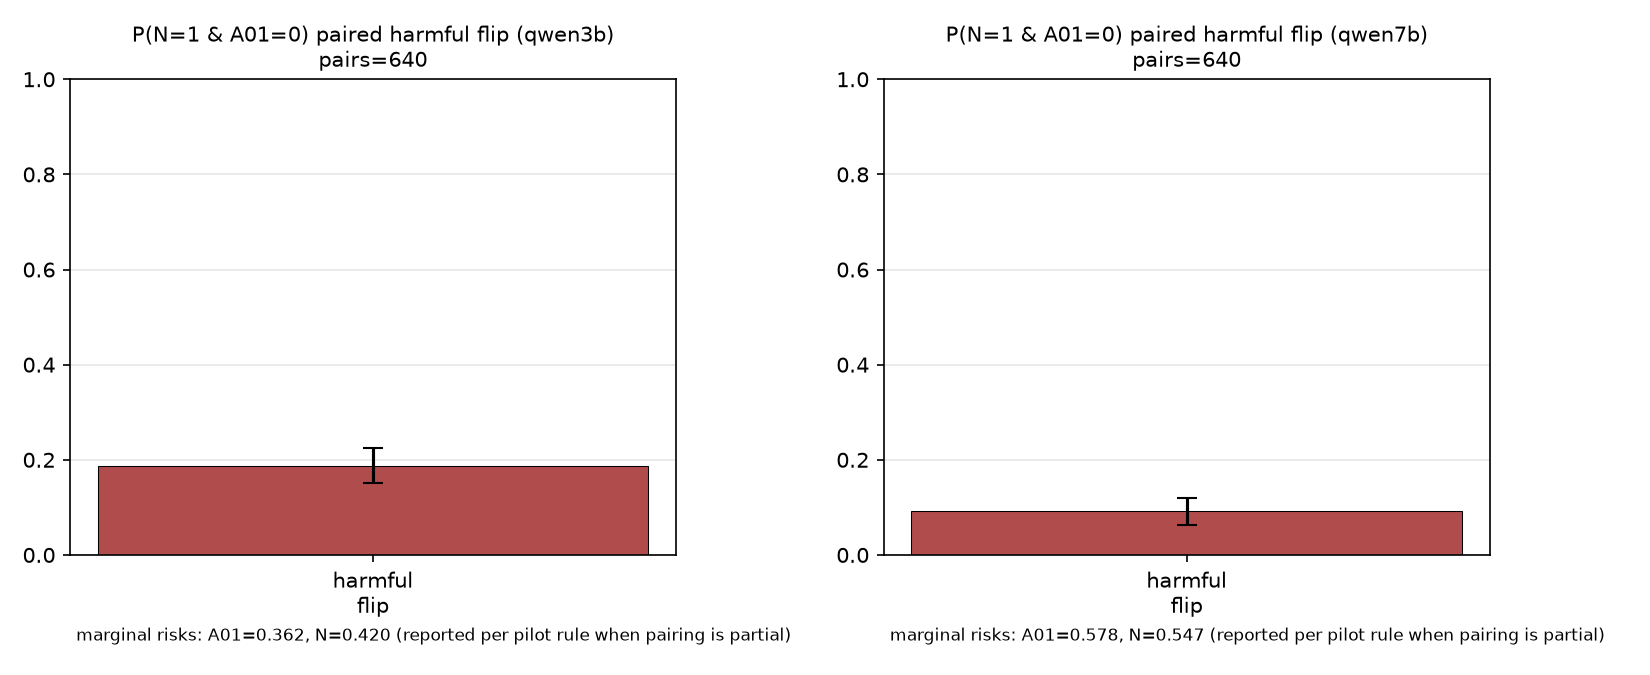
\includegraphics[width=\linewidth]{figs/fig4_harmful_flip.png}
  \caption{Paired harmful flips, A01 cell. Concentration on branches where the near-miss program semantically differs from the correct program, not a uniform effect; magnitude falls with scale.}
  \label{fig:fig4}
\end{figure}

\begin{figure}[t]
  \centering
  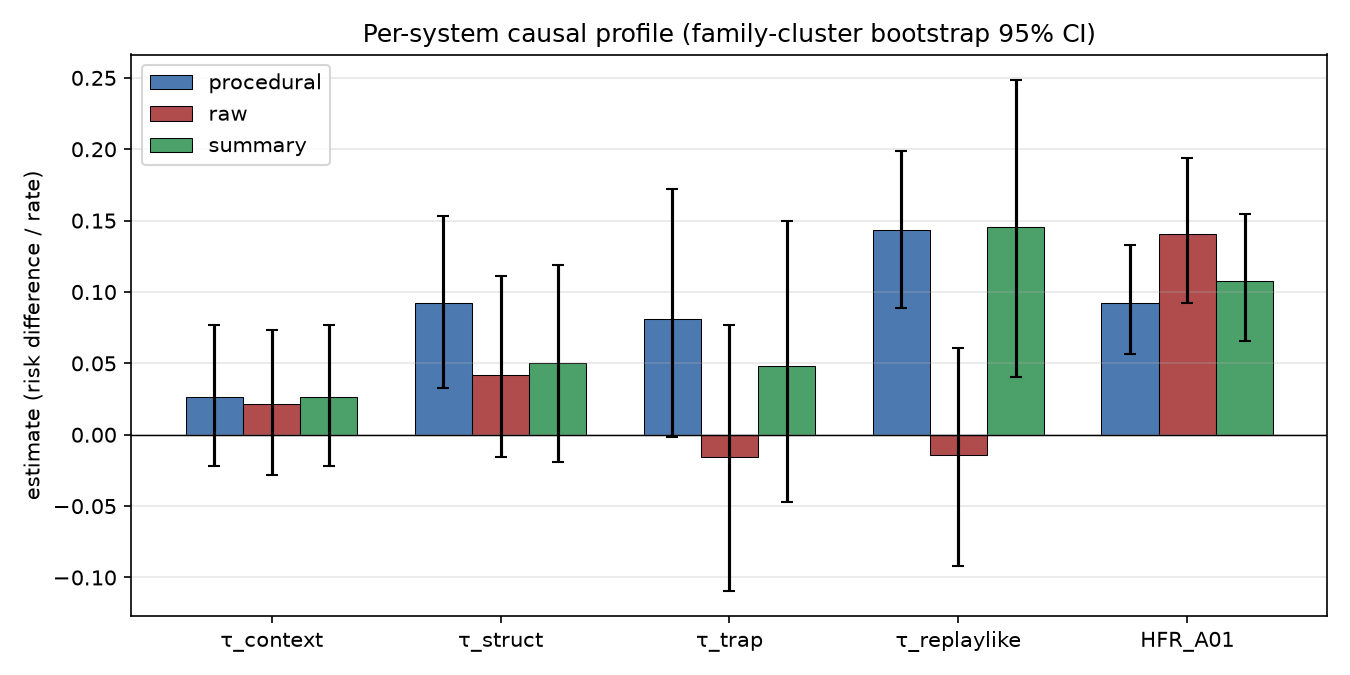
\includegraphics[width=\linewidth]{figs/hc_profiles.png}
  \caption{Form/coverage arms on fresh families (H3). Top pad: A10/A11 rates per arm; bottom pad: replay term per arm with 95\% CIs. Complete transcripts realize replay materially (TOST rejects $\pm3$pp equivalence), hard-truncated (eco) does not; form contrast is Holm-null in 8 tests.}
  \label{fig:h3}
\end{figure}

\begin{figure}[t]
  \centering
  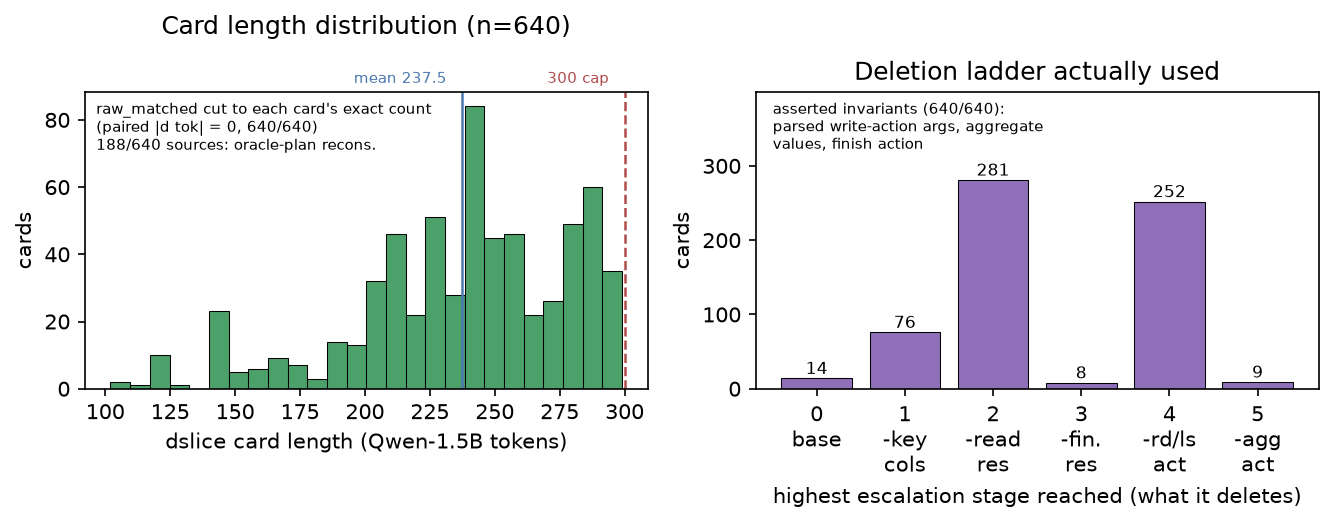
\includegraphics[width=0.92\linewidth]{figs/fig_hdc_cards.png}
  \caption{\textsc{dslice} card construction audit (Section~\ref{sec:deployment}). Left: realized card lengths (mean 237.5 tokens vs.\ the 300 cap); the paired \textsc{raw\_matched} control is cut to each card's exact count, so token budgets match per card by construction. 188/640 sources are oracle-plan reconstructions of failed harvests (provenance disclosure in \S\ref{ssec:dctest}); all arms share identical sources. Right: highest deletion stage reached per card (1: read-summary key columns; 2: read result lines; 3: finish \emph{result}; 4: non-decision action lines; 5: aggregate action lines). Asserted invariants---parsed write-action arguments, aggregate values, finish action---hold in 640/640 cards (0 QA failures).}
  \label{fig:hdccards}
\end{figure}

\begin{figure}[t]
  \centering
  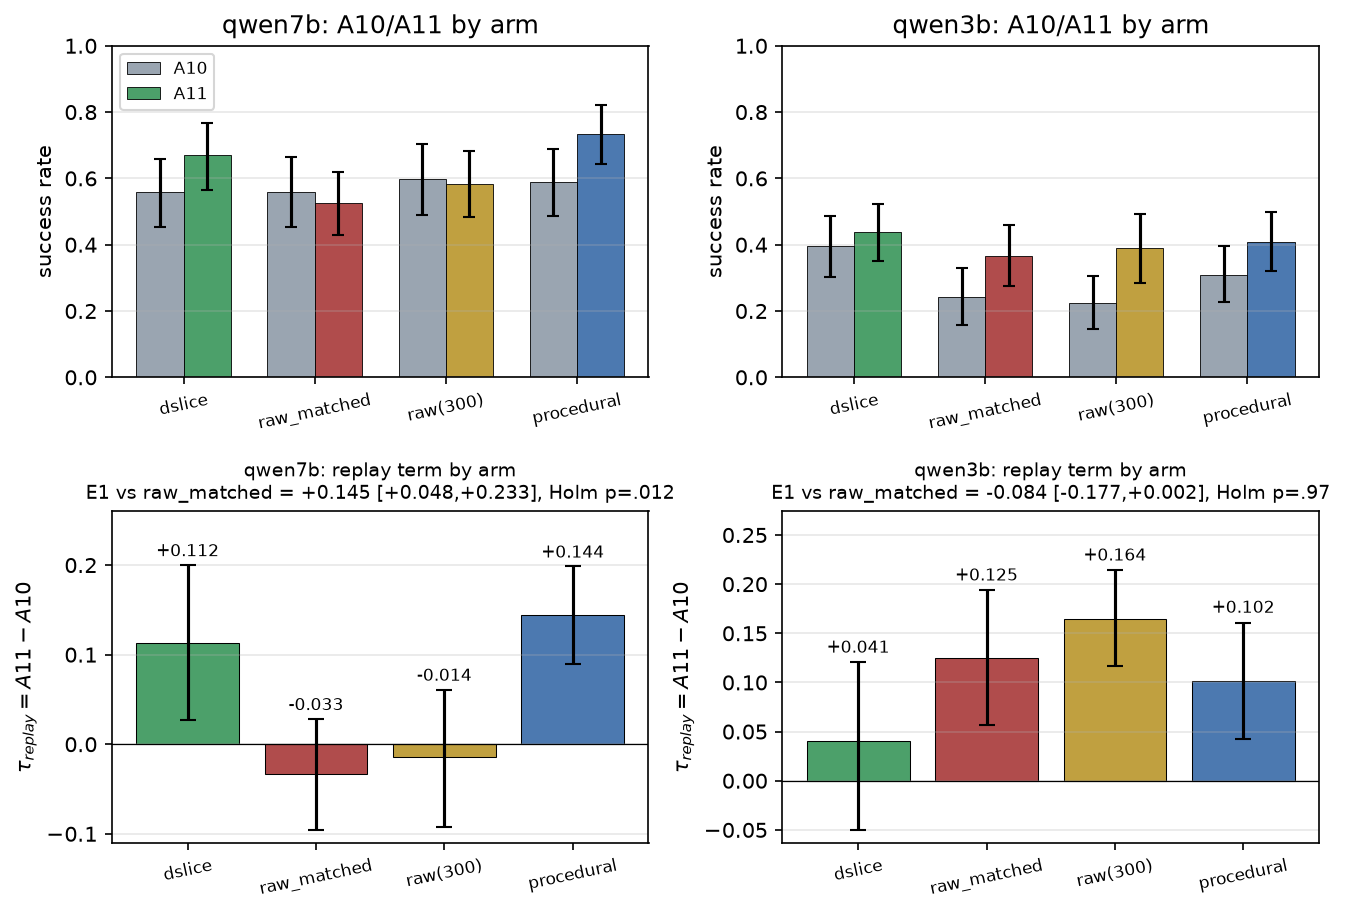
\includegraphics[width=\linewidth]{figs/fig_hdc_contrasts.png}
  \caption{Deployment result (Section~\ref{sec:deployment}). Top: A10/A11 rates per arm per model, family-cluster 95\% CIs. Bottom: replay term per arm. On the pooled 7B grid, \textsc{dslice} realizes replay while exactly-paired truncation realizes none (E1 $=+0.145$, Holm $p=.012$); at 3B there is no pooled evidence of benefit (E1 $-0.084$ [$-0.177$,$+0.002$], Holm $p=.97$). A post-hoc provenance stratification qualifies both: on authentic model-generated sources E1 $=+0.041$ [$-0.078$,$+0.149$] (7B) and $-0.226$ [$-0.347$,$-0.104$] (3B), and a direct interaction estimates oracle-minus-authentic E1 at $+0.382$ [$+0.166$,$+0.606$] (7B) and $+0.523$ [$+0.306$,$+0.783$] (3B); the pooled 7B win is carried by oracle-reconstructed sources (Appendix~\ref{app:hdc}).}
  \label{fig:hdc}
\end{figure}
